\documentclass{standalone}
\usepackage{tikz}
\begin{document}
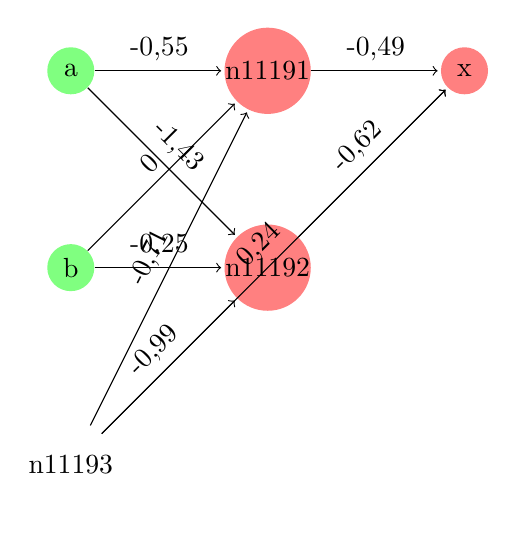
\begin{tikzpicture}[shorten >=1pt,->,draw=black!,node distance=2.5cm]
\tikzstyle{neuron}=[circle,fill=black!25,minimum size=17pt,inner sep=0pt]
\tikzstyle{constant}=[neuron, fill=white!50];
\tikzstyle{identity}=[neuron, fill=green!50];
\tikzstyle{sigmoid}=[neuron, fill=red!50];
\node [identity] (a) {a};
\node [identity,below of=a] (b) {b};
\node [constant,below of=b] (n11193) {n11193};
\node [sigmoid,right of=a] (n11191) {n11191};
\node [sigmoid,below of=n11191] (n11192) {n11192};
\node [sigmoid,right of=n11191] (x) {x};
\path[every node/.style={sloped,anchor=south,auto=false}]
(a) edge node {-1,43} (n11192)
(a) edge node {-0,55} (n11191)
(n11193) edge node {0,24} (x)
(n11193) edge node {-0,99} (n11192)
(n11193) edge node {-0,71} (n11191)
(n11191) edge node {-0,49} (x)
(b) edge node {-0,25} (n11192)
(b) edge node {0} (n11191)
(n11192) edge node {-0,62} (x)
;\end{tikzpicture}
\end{document}